\chapter{Learning latent features by capturing approximate symmetries}\label{ch:symmetries}

This chapter explores the idea of learning relational representations by identifying symmetries in data -- groups of relational objects \textit{similar} to each other, and using the obtained group membership information as latent representation of data.
The proposed approach builds upon the previously introduced relational clustering method and extends it towards the relation clustering.
This chapter is based on the following publications:

\begin{quote}
	\bibentry{DBLP:journals/corr/DumancicB16}
\end{quote}

\begin{quote}
	\bibentry{Dumancic2017}
\end{quote}

\begin{quote}
	\bibentry{Dumancic2017b}
\end{quote}




\section{Introduction}


%Every machine learning task inherently depends on the quality of provided features.
%A good set of features is thus a crucial precondition for the good performance of any classifier.
%Yet, finding such a set in practice has proven to be a tedious and time-consuming task.
%Furthermore, substantial domain knowledge and exploration are often required.
%To address this issue,  \textit{representation learning} \cite{Bengio:2009} focuses on automatic learning of good multi-level data representations.


\newglossaryentry{url}{name={URL},description={Unsupervised Representation Learning}}
Precisely defining the properties of good data representation is difficult, if not impossible.
We have seen some of the intuitive notions in Section \ref{ch3:sec:properties}, but many of them are difficult to define precisely.
Considering the case of supervised representation learning, defining a \textit{fitness} of a latent feature is somewhat possible as there is a clearly defined goal, and latent features can be assessed based on how much they help in achieving the goal.
In the case of unsupervised representation learning (URL)~\cite{Hinton504,Bengio07greedylayer-wise,RanzatoBL07}, in which the obtained representation is not tailored for one specific task but can rather be shared among multiple tasks, there is no such guidance.






To overcome this issue, \gls{url} has to resort to different means of evaluation latent features.
An interesting view on many of the \gls{url} methods is that of \textit{producing latent representation by clustering}.
Intuitively, these methods find useful features by compressing the original data by means of a  multiple-clustering procedure, in which an instance can belong to more than one cluster.
The obtained features indicate cluster assignments of instances and, thus, a classifier learns from cluster memberships instead of the original data.
For instance, auto-encoders and Restricted Boltzmann machines typically produce a sparse latent representation where each example has a small number of \textit{activated} latent features.
This can be seen as assigning examples to multiple clusterings.


A very influential work in this direction is the work of Coates and Ng \cite{coates2011analysis} that constructs a hierarchy of latent features by repeatedly clustering the data  (Figure \ref{fig:kmeansh}).
Assuming a spatial order of features (i.e., pixels), the introduced framework (i) extracts image patches, i.e., subsets of pixels from the original images candidating as a potential high-level feature, (ii) pre-processes each patch (e.g. normalisation), and (iii) learns a feature-mapping by clustering image patches.
The authors show that such general procedure with a simple k-means algorithm can perform as well as the specialised algorithms, such as auto-encoders and  Restricted Boltzmann machines.
An interesting part about this approach is that it does not require any new algorithm, but a simple adaptation of the method present in machine learning since '60s \cite{kmeans}.





\begin{figure}
	\medskip
	\centering
	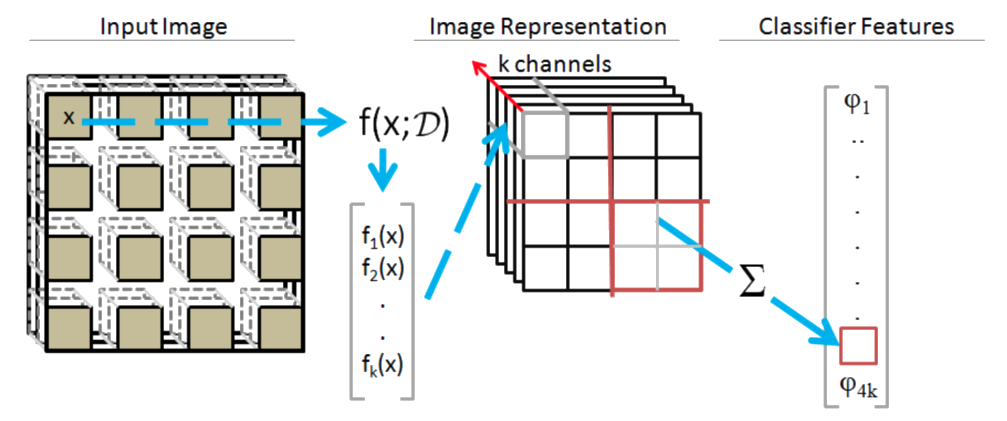
\includegraphics[width=.9\linewidth]{kmeanshierarchy}
	\caption[Learning a feature hierarchy with k-means]{\textbf{Learning a feature hierarchy with k-means.} The example images are first divided into \textit{patches}. The image patches are then clustered and centroids of the obtained clusters are used as latent features.}
	\label{fig:kmeansh}
\end{figure}



\newglossaryentry{curled}{name={CUR$^2$LED},description={Clustering-based Unsupervised Relational Representation Learning with Explicit Distributed Representation}}
%Here we focus on the problem of \textit{unsupervised} learning a \textit{feature hierarchy} with relational data.
This work introduces \gls{curled} - a \textit{clustering-based unsupervised relational representation learning with explicit distributed representation}, inspired by the work of \cite{coates2011analysis}.
The core idea behind \gls{curled} is that capturing groups of similar relational objects serve as a good \textit{proxy} for useful representations, as it identifies \textit{locally consistent} regions in example space.
All members in such a group are \textit{symmetric} to each other, meaning that for the purpose of reasoning they can be interchanged with one another.
They are approximately symmetric as they are similar, but not identical.



Though \gls{curled} is not the first approach to rely on clustering procedure to enhance the predictive performance, it posses' three distinctive features.
First, it learns a new representation by clustering both instances and their relationships.
Second, the relational structure is  preserved throughout the hierarchy, contrasted to the \gls{kge} approaches that replace relational structures with vectors.
Third, it relies on the notion of \textit{similarity interpretation}.
When clustering relational data, a similarity of relational objects is an ambiguous concept.
Two relational objects might be similar according to their attributes, relationships, or a combination of both.
The notion of similarity interpretation precisely states the exact source of similarity used.



\gls{curled} exploits this ambiguity to its advantage by using the similarity interpretations to encode a \textit{distributed representation} of data -- one of the pillars underlying the success of representation learning methods.
Intuitively, it refers to a concept of  reasonably-sized representation that captures a huge number of possible configurations \cite{Bengio2013RLR}.
In contrast to the one-hot representations which require $N$ parameters to represent $N$ regions,  distributed representations require $N$ parameters to represent up to $2^N$ regions.
The main difference is that a concept within a distributed representation is represented with several independently manipulated factors, instead of exactly one factor as with one-hot representations.
Thus, such representations are substantially more expressive.
The similarity interpretation defines the exact factors that can be manipulated individually to represent individual concepts.



The contributions of this work include
\begin{itemize}
	\item[(i)] a general framework for learning relational feature hierarchies by means of clustering
	\item[(ii)] a principled way of generating distributed relational representations based on different similarity interpretations
	\item[(iii)] a general framework for hyper-edge clustering, and
	\item[(iv)] the experimental evaluation of the proposed framework.
\end{itemize}



\section{Representation Learning via Clustering}
\label{sec:RL}

The complexity of relational data causes several issues in devising a general relational feature hierarchy: \textit{(1) what should be clustered, (2) how to estimate a similarity in relational data, and (3) how to choose the structure of a feature hierarchy? }


\paragraph{(1) What should be clustered?}
In the i.i.d. case (drawn independently from the same population), the dataset contains only instances and their features, thus, one clusters the instances.
However, relational data additionally describes relationships among instances and  varies from a single large network of many interconnected entities (a \textit{mega-example}) to a set of many disconnected networks where each network is an example.
Ideally, one would address both cases.
\gls{curled} assumes that relational data is provided as a labelled hyper-graph, where examples form vertices and relations between them form hyper-edges, and does not make a distinction between the above-mentioned cases.
Formally said, the data structure is a typed, labelled hyper-graph $H = (V,E, \tau, \lambda)$ with $V$ being a set of vertices, $E$ a set of hyper-edges, $\tau$  a function  assigning a type to each vertex and hyper-edge, and $\lambda$ a function assigning a vector of values to each vertex.
\gls{curled} learns a new representation by clustering both \textit{vertices and hyper-edges in a hyper-graph}.
Considering that vertices have associated types, \gls{curled} does not allow mixing of types, i.e., a cluster can contain only vertices of the same type.
The same holds for hyper-edges which connect vertices of different types.





\paragraph{(2) How to estimate the similarity?}
The features are the only source of similarity between instances in the i.i.d. data.
In the relational context, a similarity is an ambiguous notion that can originate in the  features of relational objects, structures of their neighbourhoods (both feature- and relationship-wise), inter-connectivity or graph proximity, just to name a few.
Furthermore, which interpretation is needed for a particular task is not known in advance, making \gls{url} inherently more difficult.
To find a representation effective for many tasks, \gls{curled} addresses \textit{multiple interpretations of relational similarity simultaneously.}
How exactly that is achieved is discussed in the next section.



\paragraph{(3) How to choose the structure?}
Defining a feature hierarchy requires the specification of the number of layers and the number of hidden features (i.e., clusters) within each layer.
How to automatically construct such hierarchies is currently under-explored.
Consequently, the performance of these methods is sensitive to the parameter setting, requiring substantial expertise in order to choose the optimal number of features.
This constitutes a major bottleneck for relational \textit{type-aware} feature hierarchies, as separate values should be chosen for each type in data (and combination thereof for hyper-edges).

To tackle this infeasibility, \gls{curled} builds upon a vast literature on \textit{the clustering selection problem} \cite{Arbelaitz:2013}, which is concerned with the selection of optimal number of clusters from data.
This automatic clustering selection strategies mitigate the problem of the manual specification of feature hierarchies.
\gls{curled} leverages  two distinct approaches: \textit{(1) a difference-like criterion} \cite{Vendramin:2010}, and \textit{(2) a quality based criterion of Silhouette index} \cite{Rousseeuw:1987}.


Difference-like criteria assess relative improvements on some relevant characteristic of the data (e.g. within-cluster similarity) over a set of successive data partitions produced by gradually increasing the number of clusters ($N$).
It attempts to identify a prominent \textit{knee} - a point when the given quality measure \textit{saturates} and the further increase of $N$ can offer only marginal benefit.
Following the suggestion in \cite{Vendramin:2010}, we choose the number of clusters as the one that achieves the highest value of the following formula:

\begin{equation}
	D(k) = \left| \frac{C(k-1) - C(k)}{C(k) - C(k+1)} \right| - \alpha \cdot k
	\label{eq:Sat}
\end{equation}

where $C(k)$ is the intra-cluster similarity, $k$ is the number of clusters and $\alpha$ a user-specified penalty on the number of clusters.


The Silhouette index evaluates a \textit{cohesion}, i.e., how similar an instance is to its own cluster, and a \textit{separation}, i.e., how similar an instance is to the other clusters.
It is defined as:

\begin{equation}
    S(i) = \frac{a(i) - b(i)}{ \max \{ a(i), b(i)\}}
\end{equation}

where $i$ is an instance, $a(i)$ is an average dissimilarity of $i$ to the rest of the instances in the same cluster, and $b(i)$ the lowest dissimilarity of $i$ to any other cluster.
Higher values indicate a better fit of the data.


\begin{sidewaysfigure}
  \centering
  \medskip
  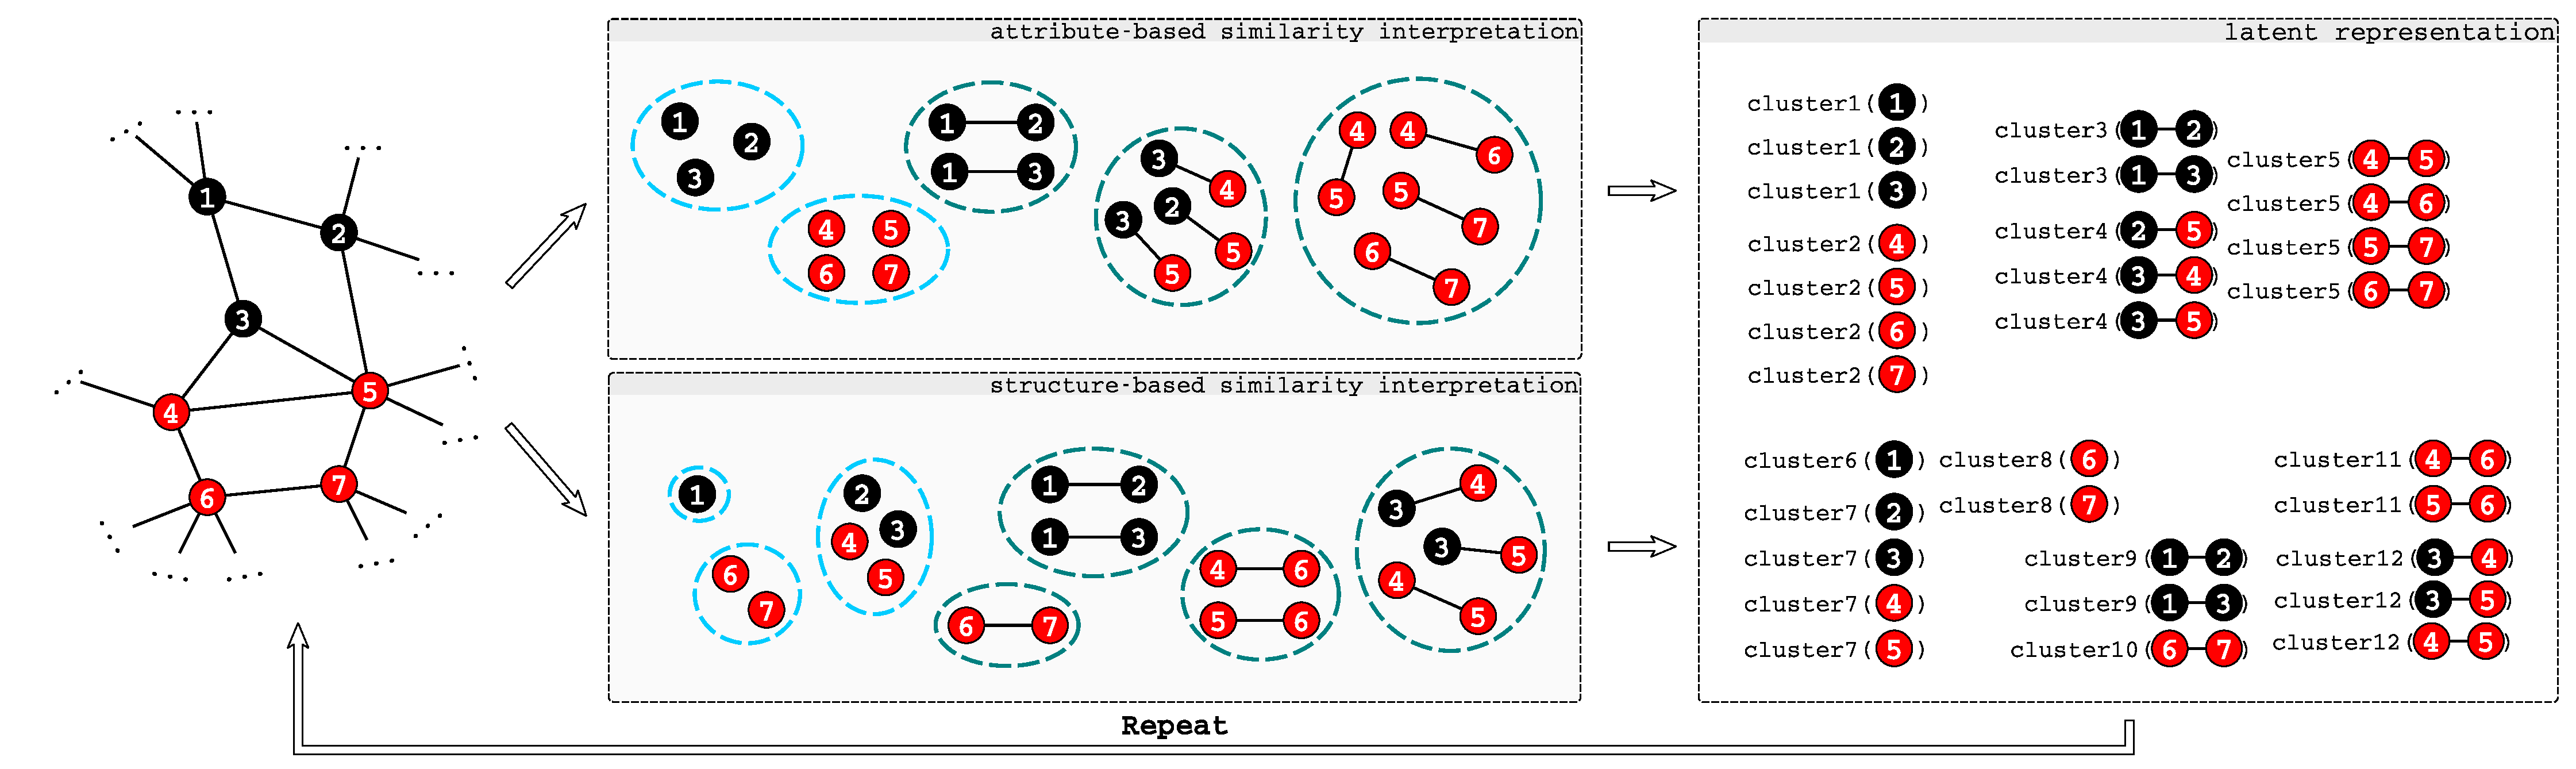
\includegraphics[width=.99\textwidth]{curled}
  \caption[An illustration of \gls{curled} procedure]{\textbf{An illustration of \gls{curled} procedure.} The left-most figure represents a given hyper-graph, where colour of a vertex indicates its feature value. The graph (i.e., vertices and edges) is then clustered according to different similarity interpretations. The upper clustering is based on vertex attributes: the vertices are clustered into \textit{red} and \textit{black} ones, while the edges are clustered according to the colour of the vertices they connect. The bottom clustering is based on the structure of the neighbourhoods. The vertices are clustered into a group that have only \textit{black} neighbours (\{{\tt1}\}), only \textit{red} neighbours (\{\texttt{6,7}\}), and neighbours of both colours (\{\texttt{2,3,4,5}\}). The edges are clustered into a group of edges connecting \textit{black} vertices with only \textit{black} neighbours and \textit{black} vertices with \textit{red} neighbours (\{\texttt{1-2,1-3}\}), a group of edges connecting \textit{red} vertices with only \textit{red} neighbours to \textit{red} vertices with neighbours of both colour (\{\texttt{6-7}\}), and so on. The final step transforms the obtained clusterings into a relational representation. The procedure can further be repeated to create more layers of features. }
  \label{fig:curled}
\end{sidewaysfigure}


\textbf{$\mathcal{C}$-representation.}
Once the clusters are obtained, we will represent them in the following form.
For each cluster of vertices we create a unary predicate in the form of \texttt{cluster$ID$(vertex)} where \texttt{vertex} is an identifier of a specific vertex.
Similarly, for each cluster of hyper-edges we create a $n$-ary predicate in the form of \texttt{cluster$ID$(vertex$_1$,\ldots,vertex$_n$)}, which takes an ordered set of $n$ vertices as arguments.
Truth instantiations of defined predicates reflect cluster memberships.
We refer to the cluster-induced representation as a $\mathcal{C}$-representation.





The introduced pipeline is illustrated in Figure~\ref{fig:curled}.
\gls{curled} specified thus far describes a \textit{meta-procedure} how to use any clustering algorithm to obtain a latent representation.
In the experiments we use spectral and hierarchical clustering.



\section{Similarity of Relational Structures}
\label{sec:Clustering}


\gls{curled} relies on the previously introduced approach \gls{recent}.
What makes \gls{recent} an attractive relational clustering framework is the wide range of similarities it considers.
We will refer to them as \textit{core similarities}.
Furthermore, which similarity is used is easily adaptable with just a few parameters.
%We provide a concise and intuitive description here, and refer the reader to the original paper for the details.


%The core concept of ReCeNT is a \textit{neighbourhood tree} (NT).
%The NT is a rooted directed graph describing a neighbourhood of a certain vertex in the hyper-graph.
%It provides a summary of all paths that can be taken, starting from that particular vertex.
%The depth of a NT, i.e., how many vertices a path can contain excluding the root vertex, is pre-specified.
%ReCeNT compares two vertices by comparing their NTs.



%This comparison is achieved by first decomposing the NT into different multisets.
%The multiset $V^l_{t}(g)$ contains all vertices of type $t$ at distance $l$ of a particular NT $g$.
%$E^l(g)$ is the multiset of hyper-edge labels between vertices of distances $l$ and $l+1$.
%Finally, $B^l_{t,a}(g)$ is the multiset of values of attribute $a$ observed among the nodes of type $t$ at distance $l$.
%Using only these three types of multisets, one can express a wide range of similarities.
%What ReCeNT considers are:
%\begin{enumerate}
%    \item the similarity of the root vertices in terms of attribute values, by means of $B^0_{t,a}$
%    \item the similarity of attribute values of the neighbouring vertices, by means of $B^{l>0}_{t,a}$
%    \item the connectivity of the root vertices, by means of $V^l_t$
%    \item the similarity of neighbourhoods in terms of the vertex identities, by means of $V^l_t$
%    \item the similarity of hyper-edge labels of two neighbourhoods, by means of $E^l$.
%\end{enumerate}


%Each of the components represents a distinct notion of similarity.
%We will refer to them as \textit{core similarities}.
%These core similarities can further be combined to represent more complex similarities.


\subsection{Hyper-edge Similarity}

\newglossaryentry{nt}{name={NT},description={Neighbourhood tree}}
In its original form, \gls{recent} clusters vertices in a hyper-graph.
To support hyper-edge clustering with \gls{curled}, we introduce a general framework for hyper-edge similarity.
It views hyper-edges as ordered sets of vertices, and thus ordered sets of neighbourhood trees (\gls{nt}s).


Let $\mathcal{N}$ be a set of \gls{nt}s.
Let $\Theta$ denote summary operations on sets of values such as mean, minimum and maximum.
Let $\Lambda$ denote set operators such as union and intersection.
Let $f: \mathcal{N}^2 \rightarrow \mathbb{R}$ be a similarity between two \gls{nt}s, e.g. the similarity measure introduced by \gls{recent}.
The framework introduces two types of hyper-edge similarity, namely \textit{combination} and \textit{merging}.


\begin{definition}
A \textit{combination similarity} is a function $c: \mathcal{N}^n \times \mathcal{N}^n \times \Theta \rightarrow \mathbb{R}$ which compares two hyper-edges, $e_1 = (v_1^1,..., v_1^n)$ and $e_1 = (v_2^1,..., v_2^n)$, by comparing the individual \gls{nt}s respecting the order, $s = \left(f(v_1^1,v_2^1),\ldots,f(v_1^i,v_2^i) \right)$, and summarising respective similarities with $\theta \in \Theta$,  $\theta(s)$.
\end{definition}

\begin{definition}
A \textit{merging similarity} is a function $m: 2^{\mathcal{N}} \times 2^{\mathcal{N}} \times \Lambda \rightarrow \mathbb{R}$ which compares two hyper-edges, $e_1 = (v_1^1,..., v_1^n)$ and $e_1 = (v_2^1,..., v_2^n)$, by first merging the \gls{nt}s within a hyper-edge with merging operator $\lambda \in \Lambda$, $s_1 = \lambda (v_1^1,\ldots,v_1^i)$ and $s_2 = \lambda (v_2^1,\ldots,v_2^i)$ and comparing the resulting gls{nt}s, $f(s_1,s_2)$.
\end{definition}


Merging two \gls{nt}s involves merging their respecting multi-sets with a merging operator $\lambda$, respecting the level.
For instance, consider \textit{set union} as $\lambda$, and $g'$ and $g''$ as the \gls{nt}s to be merged.
Then, merging the multi-sets $V^l_{t}(g')$ and $V^l_{t}(g'')$ results in a multi-set $V^l_{t}\left(\lambda(g',g'')\right) = V^l_{t}(g') \cup V^l_{t}(g'')$.


\begin{figure}
	\centering
	\begin{subfigure}{\linewidth}
		\centering
		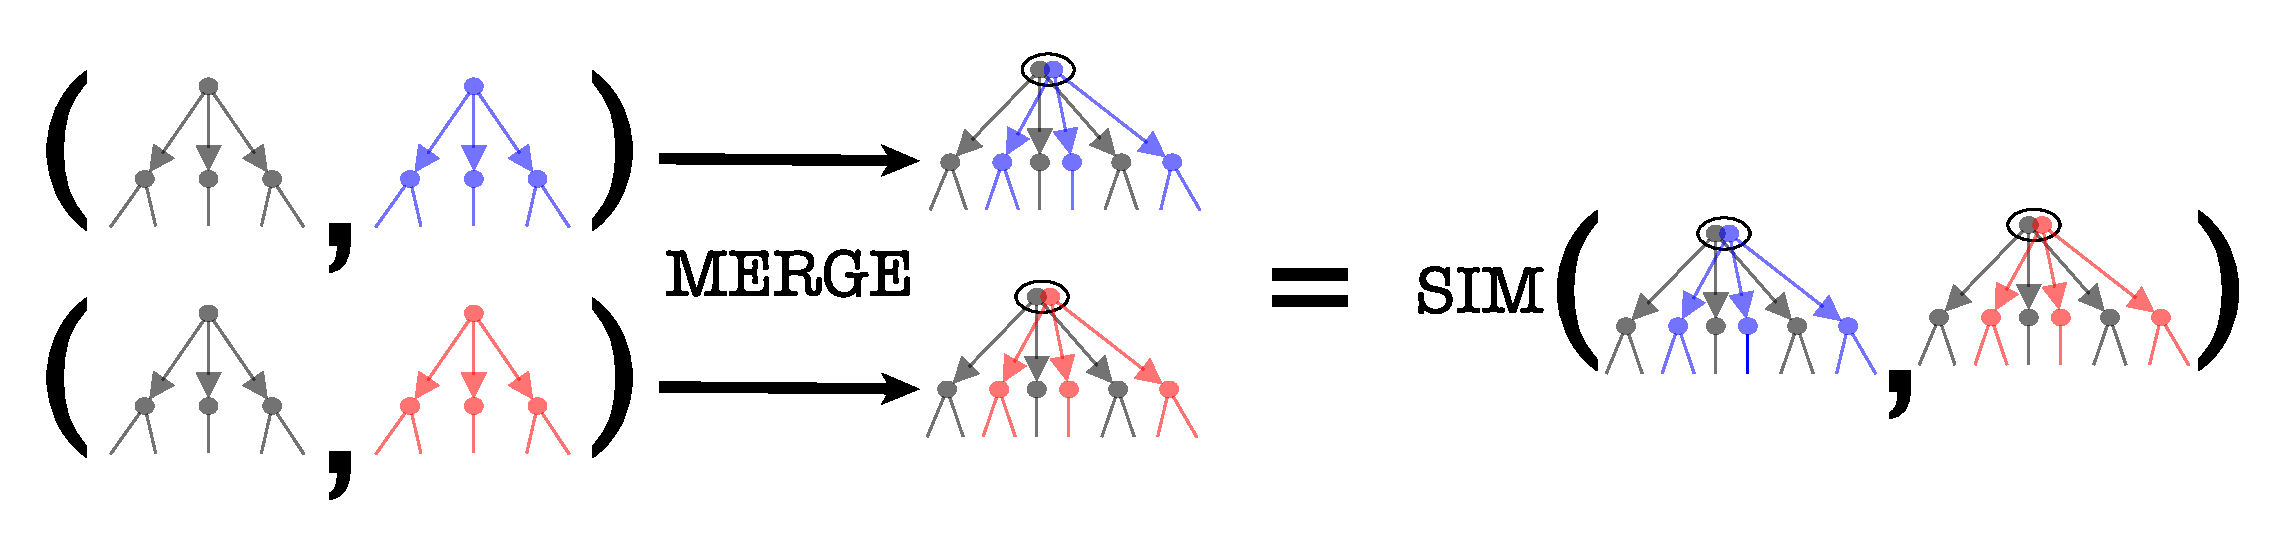
\includegraphics[width=.85\linewidth]{merging}
		\caption{Merging neighbourhood trees\label{fig:ntmerging}}
	\end{subfigure}

	\begin{subfigure}{\linewidth}
		\centering
		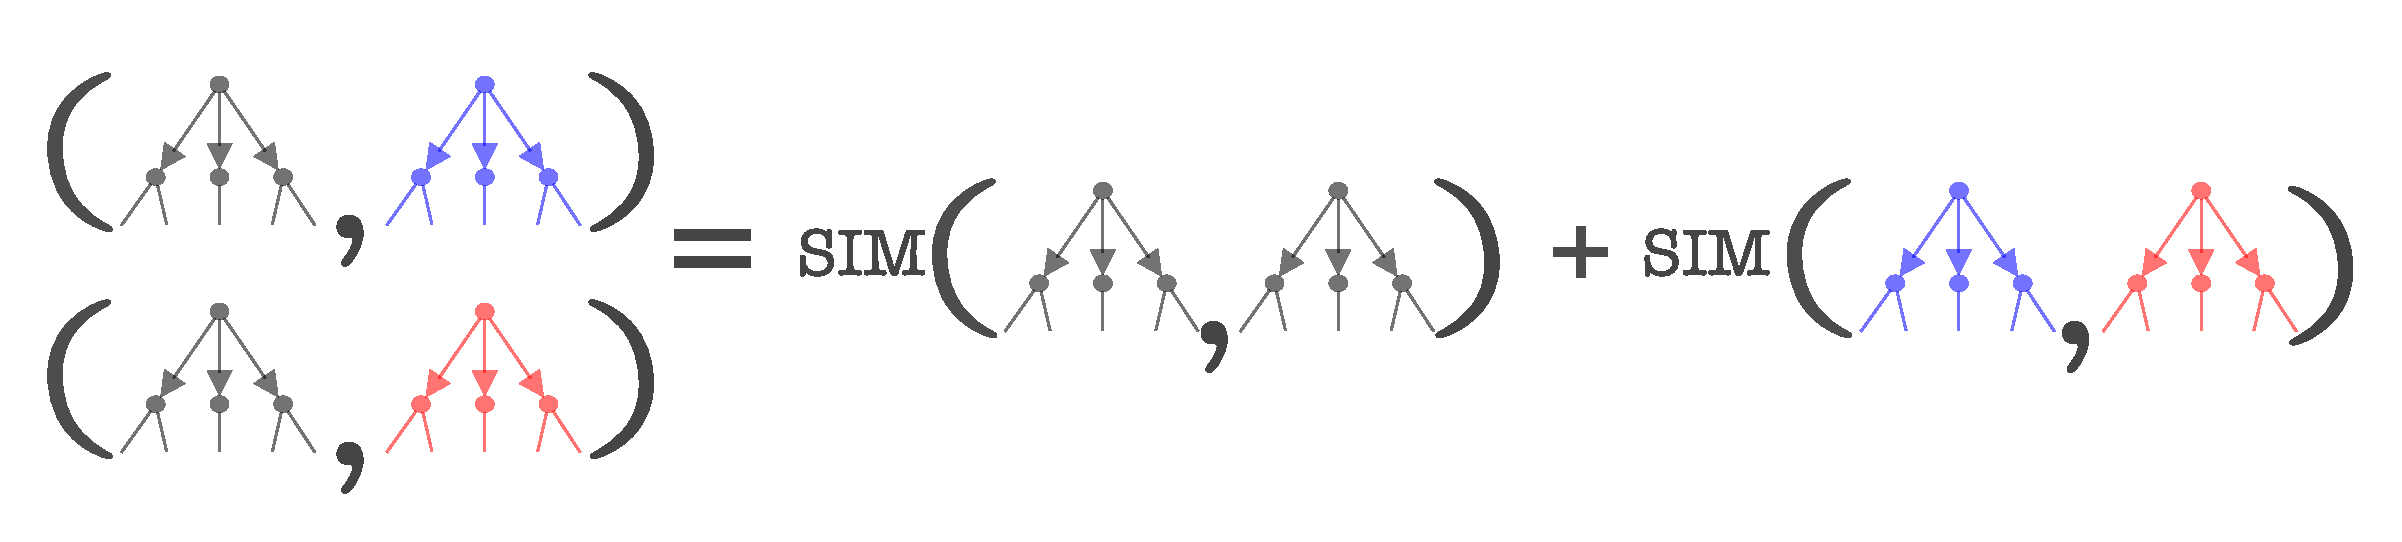
\includegraphics[width=.85\linewidth]{combination}
		\caption{Combining neighbourhood trees\label{fig:ntcombination}}
	\end{subfigure}
	\caption{Illustration of hyper-edge similarity operators}
\end{figure}


Both formulations reduce the problem to the comparison of \gls{nt}s, but offer alternative views.
While \textit{merging} ignores the order of vertices in a hyper-edge, \textit{combination} respects it.
Accordingly, \textit{merging} describes the neighbourhood of a hyper-edge, while \textit{combination} examines the similarity of vertices participating in a hyper-edge.
In this work we use \textit{union} as the merging operator, and \textit{mean} as the combination operator.



\subsection{Similarity Interpretation}

Finally, we formally introduce the notion of similarity interpretation.

\begin{definition}
Let $(w_1,w_2,w_3,w_4,w_5)$ be the weights associated with the \textit{core similarities}.
A \textit{similarity interpretation} is the value assignments to the weights $(w_1,w_2,w_3,w_4,w_5)$.
\end{definition}

Thus, it allows us to precisely control aspects of similarity considered for representation learning.
For example, setting $w_1 = 1, w_{2,3,4,5} = 0$ uses only the attributes of vertices for comparison.
Setting $w_3 = 1, w_{1,2,4,5} = 0$ on the other hand would identify clusters as a densely connected components.
As the similarity interpretation is provided by the user, we say it \textit{explicitly} defines the distributed representation.




\section{Related Work}
\label{sec:Related}

Clustering has been previously recognised as an effective way of enhancing relational learners.
\cite{Popescul2004}  apply k-means clustering to instances, create predicates for new clusters and add them to the original data.
\textit{Multiple relational clustering (MRC)} \cite{Kok2007,Kok2008} is a relational probabilistic clustering framework based on Markov logic networks \cite{Richardson2006} clustering both vertices and relationships.
Both approaches are instances of predicate invention \cite{Kramer1995,Craven2001}, concerned with extending the vocabulary given to a learner by discovering novel concepts in data.
\gls{curled} differs in several ways.
Whereas \cite{Popescul2004} develop a method specifically  for document classification, \gls{curled} is a general \textit{off-the-shelf} procedure that can be applied to any relational domain.
Moreover, CUR$^2$LED clusters both instances and relations, whereas \cite{Popescul2004} cluster only instances.
In contrast to MRC which does not put any assumptions in the model, \gls{curled} is a more informed approach that explicitly defines different notions of relational similarity to be used for clustering.
Though MRC was used as a component in structure learning, it does not provide new language constructs, but simplifies the search over possible formulas.
\gls{curled} learns a model directly from the new features.


A related problem is community detection \cite{Karypis:1998:FHQ:305219.305248,Fortunato201075} concerned with identifying a densely connected components in graphs.
\gls{curled} considers a more general problem in which \textit{disconnected} vertices (and edges) can form clusters as well.


% Much of the recent work focused on  \textit{embedding} relational data into \textit{vector spaces} \cite{Nickel0TG16,DBLP:conf/nips/Niepert16,Bordes:2011:LSE,Bordes:2013:TEM,DBLP:conf/icml/NiepertAK16}.
% The essential idea behind these approaches is to map relational concepts to a low-dimensional vectors spaces, and replace logical reasoning with algebra.
%The drawbacks of these approaches is that the latent features are not interpretable, don't preserve the relational information and require huge amounts of data.
On contrast to the various \gls{kge} methods that invent an Euclidean space of relational instances, \gls{curled} relies on clustering and a variety of similarity measures to create new features.


\section{Experiments and Results}
\label{sec:Results}




\textbf{Datasets.}
We have used the following six datasets to evaluate the potential of this approach.
The IMDB dataset describes a set of movies with people acting in or directing them.
The UW-CSE dataset describes the interactions of employees at the University of Washington and their roles, publications and the courses they teach.
The Mutagenesis dataset describes chemical compounds and atoms they consist of.
The WebKB dataset consists of pages and links collected from the Cornell University's web page.
The Terrorists dataset describes terrorist attacks each assigned one of 6 labels indicating the type of the attack.
The Hepatitis dataset describes a set of patients with hepatitis types B and C.


\textbf{Evaluation procedure.}
In principle, a latent representation should make learning easier by capturing complex dependencies in data more explicitly.
Though that is difficult to formalise, a consequence should be that a model learned on the latent representation is (i) \textit{less complex}, and (ii) possibly \textit{performs better}.
To verify whether that is the case with the representation created by \gls{curled}, we answer the following questions:
\begin{itemize}
	\setlength\itemsep{0.06em}
    \item[\textbf{(Q1)}] \textit{do representations learned by \gls{curled} induce models of lower complexity compared to the ones induced on the original representation?}
    \item[\textbf{(Q2)}] \textit{if the original data representation is sufficient to solve a task efficiently, does $\mathcal{C}$-representation preserves the relevant information?}
    \item[\textbf{(Q3)}] \textit{if the original data representation is not sufficient to solve the task, does a $\mathcal{C}$-representation improve the performance of a relational classifier?}
    \item[\textbf{(Q4)}] \textit{can the appropriate parameters for a specific dataset be found by the model selection?}
    \item[\textbf{(Q5)}] \textit{how does \gls{curled} compare to MRC, which is the closest related work?}
\end{itemize}


\newglossaryentry{tilde}{name={TILDE},description={Top-Down Induction of Logical Decision Trees}}
In order to do so, we use \gls{tilde} \cite{Blockeel1998285}, a relational decision tree learner, and perform leave-one-out cross validation.
$\mathcal{C}$-representations and \gls{tilde} were learned on training folds, and the objects from the test fold were mapped to the $\mathcal{C}$-representation and used to test \gls{tilde}.
The following similarity interpretation were used for each dataset: (0.5,0.5,0.0,0.0,0.0), (0.0,0.0,0.33,0.33,0.34), (0.2,0.2,0.2,0.2,0.2).
The first set of weights uses only the attribute information, the second one only the link information, while the last one combines every component.



As a complexity measure of a model we use the number of nodes a trained \gls{tilde} model has.
We use the following values for the $\alpha$ parameter in Equation~\ref{eq:Sat}: $\{ 0.1,0.05, 0.01 \}$.
In the case of MRC, we used the following values for the $\lambda$ parameter: $\{-1,-5,-10\}$.
The $\lambda$ parameter has the same role as $\alpha$ in the proposed approach, affecting the number of clusters chosen for each type\footnote{Note that it is difficult to exactly match the values of $\alpha$ and $\lambda$ as both methods operate on different scales, and the authors do not provide a way how to choose an appropriate value}.




\subsection*{Results}


\begin{table*}
\captionsetup{justification=centerlast}
    \begin{center}
        \footnotesize
        \caption[Performance of \gls{tilde} models learned on the original and latent representations.]{\textbf{Performance comparison for TILDE models learned on the original and $\mathcal{C}$-representations.} The first column specifies the parameters used for $\mathcal{C}$-representation, i.e., clustering algorithm (S-spectral, H-hierarchical), selection criterion and its parameter values. Both accuracies on a test set (Acc) and complexities (Cplx) are reported.}
        \resizebox{0.98\textwidth}{!}{%
        \begin{tabular}[th]{@{}lrrrrrrrrrrrrr@{}}
            \toprule
                \multirow{2}{*}{}& \multirow{2}{*}{\textbf{Setup}} & \multicolumn{2}{r}{\textbf{IMDB}} & \multicolumn{2}{r}{\textbf{UWCSE}} & \multicolumn{2}{r}{\textbf{Mutagenesis}} & \multicolumn{2}{r}{\textbf{Terrorists}} & \multicolumn{2}{r}{\textbf{Hepatitis}} & \multicolumn{2}{r}{\textbf{WebKB}} \\
								\cmidrule(lr){3-4} \cmidrule(lr){5-6} \cmidrule(lr){7-8} \cmidrule(lr){9-10} \cmidrule(lr){11-12} \cmidrule(l){13-14}
                                 &                                 &  Acc & Cplx &  Acc & Cplx & Acc & Cplx & Acc & Cplx & Acc & Cplx & Acc & Cplx \\
                \midrule

                                 & \textbf{Original}                                                    & 1.0  & 2.0        & 0.99 & 3.0                & 0.76 & 27.2                   & \textbf{0.72} & 86.4       & 0.81 & 22.4       & 0.81 & 18.2 \\
               \midrule
       \parbox[t]{2mm}{\multirow{8}{*}{\rotatebox[origin=c]{90}{\textbf{merging}}}} & S,$\alpha=0.01$   & 1.0  & 1.0        & 0.99 & 1.2                 & 0.79 & 6.6                   & \textbf{0.71} & 34.4       & 0.86 & 19.66             & \textbf{0.89 }& 13.6  \\

                                                                                    & S,$\alpha=0.05$   & 1.0  & 1.0        & 0.99 & \textbf{1.0}        & 0.78 & 2.4                   & 0.65 & 21.6                & 0.90 & 7.6                & 0.85 & 15.6 \\

                                                                                    & S,$\alpha=0.1$    & 1.0  & 1.0        & 0.99 & 1.2                 & 0.78 & \textbf{1.8}          & 0.66 & 32.4                & 0.90 & 6.5               & \textbf{0.87} & 17.8  \\

                                                                                    & S,silhouette      & 1.0  & 1.0        & 0.99 & \textbf{1.0}        & 0.78 & \textbf{2.0}          & 0.6 & 23.6                 & \textbf{0.93} & \textbf{5.33}       & \textbf{0.87} & 14.8 \\

                                                                                    & H,$\alpha=0.01$   & 1.0  & 1.0        & 0.98 & 4.4                 & \textbf{0.83} & \textbf{2.0} & 0.48 & \textbf{9.4}        & 0.86 & 12.0       & 0.83 & 12.6  \\

                                                                                    & H,$\alpha=0.05$   & 1.0  & 1.0        & 0.99 & 4.2                 & \textbf{0.83} & \textbf{2.0} & 0.48 & 11.6                & 0.82 & 16.0       & 0.69 & 27.2 \\

                                                                                    & H,$\alpha=0.1$    & 1.0  & 1.0        & 0.99 & 4.0                 & 0.79 & 5.2                   & 0.47 & \textbf{8.8}        & 0.82 & 13.4       & 0.61 & 32.2 \\

                                                                                    & H,silhouette      & 1.0  & 1.0        & 0.98 & \textbf{1.0}        & 0.80 & 3.4                   & 0.47 & 13.0                & \textbf{0.93} & 8.66       & 0.68 & 18.0 \\
                \midrule
   \parbox[t]{2mm}{\multirow{8}{*}{\rotatebox[origin=c]{90}{\textbf{combination}}}} & S,$\alpha=0.01$   & 1.0  & 1.0        & 0.99 & 1.2                 & 0.79 & \textbf{2.0}          & \textbf{0.72} & 24.0       & 0.90 & 7.6        & \textbf{0.90} & 11.8 \\

                                                                                    & S,$\alpha=0.05$   & 1.0  & 1.0        & 0.99 & \textbf{1.0}        & 0.79 & \textbf{2.0}          & 0.69 & 22.8                & 0.88 & 12.2       & 0.86 & \textbf{10.0} \\

                                                                                    & S,$\alpha=0.1$    & 1.0  & 1.0        & 1.0 & \textbf{1.0}         & 0.76 & \textbf{2.0}          & 0.66 & 16.8                & 0.90 & 12.6       & 0.87 & 17.0 \\

                                                                                    & S,silhouette      & 1.0  & 1.0        & 0.99 & \textbf{1.0}        & 0.77 & \textbf{2.0}          & 0.6  & 24.2                & \textbf{0.93} & 16.4       & \textbf{0.88} & 13.8\\

                                                                                    & H,$\alpha=0.01$   & 1.0  & 1.0        & 0.99 & 2.8                 & 0.79 & 4.0                   & 0.51 & 30.6                & 0.80 & 29.33      & 0.83 & 12.6 \\

                                                                                    & H,$\alpha=0.05$   & 1.0  & 1.0        & 0.99 & 2.8                 & 0.78 & 2.8                   & 0.51 & 30.6                & 0.82 & 16.33      & 0.69 & 27.2 \\

                                                                                    & H,$\alpha=0.1$    & 1.0  & 1.0        & 0.99 & 2.8                 & 0.78 & 11.0                  & 0.50 & 27.3                & 0.78 & 14.0       & 0.61 & 32.2   \\

                                                                                    & H,silhouette      & 1.0  & 1.0        & 0.99 & 2.0                 & 0.80 & 4.0                   & 0.50 & 30.0                & 0.83 & 11.6       & 0.68 & 18.0  \\
                \midrule
        \parbox[t]{2mm}{\multirow{3}{*}{\rotatebox[origin=c]{90}{\textbf{MRC}}}}    & $\lambda=-1$      & 1.0  & 1.0       & 0.93 & 21.0        & 0.6  & 0          & 0.64 & 138.7      &  0.61 & 99.4        &0.64 & 44.4 \\

                                                                                    & $\lambda=-5$      & 1.0  & 1.0       & 0.95 & 25.9        & 0.63  & 23.5      & 0.50 & 126.5        & 0.84 & 64.8       &0.68 & 40.0 \\

                                                                                    & $\lambda=-10$     & 1.0  & 1.0       & 0.96 & 13.7        & 0.72  & 35.0      & 0.51 & 102.1        & 0.57 & 5.7         &0.66 & 40.8 \\
                \bottomrule



        \end{tabular}
        }
        \label{tab:Results}
    \end{center}
\end{table*}


To answer the above mentioned questions, we perform two types of experiments.
Table~\ref{tab:Results} summarises the results of cross validation.
The accuracies on test set and the complexities of \gls{tilde} models are stated for both original and $\mathcal{C}$-representations.
Table~\ref{tab:MS} summarises the results of the model selection where we dedicate one fold as a \textit{validation set}, and perform the cross validation on the remaining folds to identify the best parameter values (i.e., the choice of a clustering algorithm, a clustering selection procedure and the appropriate hyper-edge similarity) for each dataset.

\textbf{Q1.}
Table~\ref{tab:Results} shows that the models learned on $\mathfrak{C}$-representation consistently have lower complexity than the ones learned on the original data.
That is especially the case when $\mathcal{C}$-representation is obtained by spectral clustering, which consistently results in a model of a lower complexity.
The reduction of complexity can even be surprisingly substantial, for instance on the Mutagenesis and Hepatitis datasets where the model complexities are reduced by factors of 10 and 4, respectively.
When the $\mathcal{C}$-representation is obtained with hierarchical clustering, models of lower complexity are obtained on all datasets except the WebKB and UWCSE datasets.
These results suggest that the $\mathcal{C}$-representation in general makes complex dependencies easier to detect and express.




\textbf{Q2.}
The IMDB and UWCSE datasets are considered as \textit{easy} relational datasets, where the classes are separable by a single attribute or a relationship.
Thus, TILDE is able to achieve almost perfect performance  with the original data.
The original representation is therefore sufficient to solve the task, and we are interested whether  the relevant information will be preserved within the $\mathcal{C}$-representation.
The results in Table~\ref{tab:Results} do suggest so, as \gls{tilde} achieves identical performance regardless of the representation.



\textbf{Q3.}
The remaining datasets are more difficult than the previously discussed ones.
On the Mutagenesis, Hepatitis and WebKB datasets, $\mathcal{C}$-representation improves the performance.
On the Terrorists dataset, however, no improvement in performance is observed.
What distinguishes this dataset from the others is that it contains only two edge types (indicating co-located attack, or ones organised by the same organisation), an abundant number of features, while other datasets are substantially more interconnected.
Thus, focusing on the relational information is not as beneficial as the features themselves.

These results suggest that $\mathcal{C}$-representations indeed improve performance of the classifier, compared to the one learned on the original data representation.
First, the $\mathcal{C}$-representation created with spectral clustering consistently performs better on all datasets, except the Terrorists one.
Second, if the learning  task does not have a strong relational component, then $\mathcal{C}$-representations are not beneficial and can even hurt the performance (this is the case with the Terrorists dataset).
Third, the choice of a clustering algorithm matters, and spectral clustering does a better job in our experiments - it always results in improved or at least equally good performance.
Fourth, the choice of treating hyper-edges as ordered (by \textit{combination}) or un-ordered (\textit{merging}) sets is data-dependent, and the difference in performance is observed.


Combining the results from \textbf{Q1}, \textbf{Q2} and \textbf{Q3} shows that \textit{the main benefit} of \gls{curled} is \textit{the transformation of data such that it becomes easier to express complex dependencies}.
Consequently, the obtained models have lower complexities and  their performance often improves.


\textbf{Q4.} To ensure that the previously discussed results do not over-fit the data, we additionally perform model selection.
We dedicate one fold as the \textit{validation set}, and use the remaining folds to find the best parameter values of both \gls{curled} and \gls{tilde}.
Table \ref{tab:MS} summarises the results and reports the selected choice of parameter, together with the performance on the validation set.
These results are consistent with the ones in Table~\ref{tab:Results}: $\mathcal{C}$-representation improves the performance in the majority of cases, and the selected parameters correspond to the best performing ones in Table~\ref{tab:Results}.

\begin{table}
	\centering
\captionsetup{justification=centerlast}

	\caption[Model selection results with TILDE and \gls{curled}]{\textbf{Model selection results.} For each dataset, a selected parameters are reported together with the accuracies on the training and test sets. The first element indicates the selected clustering algorithm (S-spectral, H-hierarchical), the second one the clustering selection criteria, while the last one indicates the hyper-edge similarity (C-combination, M-merging). The last column indicates the performance on the original data representation. }
    \resizebox{0.8\linewidth}{!}{%
    	\begin{tabular}[t]{ccccc}
        \toprule
        \textbf{Dataset} & \textbf{Parameters} & \textbf{Training} & \textbf{Validation} & \textbf{Original}\\
        \midrule
        \textbf{IMDB} & all & 1.0 & \textbf{1.0} & \textbf{1.0}\\

        \textbf{UWCSE} & S, silhouette, C & 0.99 & \textbf{1.0} & 0.99 \\

        \textbf{Mutagenesis} & H, $\alpha$=0.01, M & 0.86 & \textbf{0.84} & 0.79 \\

        \textbf{Hepatitis} & S, silhouette, M & 0.92 & \textbf{0.89} & 0.8  \\

        \textbf{WebKB} & S, $\alpha$=0.01, C & 0.88 & \textbf{0.88} & 0.79 \\

        \textbf{Terrorists} & S,$\alpha$=0.01, C & 0.70 & 0.69 & \textbf{0.71} \\
        \bottomrule
        \end{tabular}

    }
    \label{tab:MS}

\end{table}




\textbf{Q5.}
Table~\ref{tab:Results} shows that \gls{curled} substantially outperforms MRC on all datasets, achieving better performance on all datasets except the IMDB.
Moreover, MRC rarely shows benefit over the original data representation, with an exception on the Hepatitis dataset.
Considering the model complexity, the models learned on MRC-induced representation are substantially more complex than the ones learned on $\mathcal{C}$-representations.
Table~\ref{tab:Size} summarise the number of clusters created by \gls{curled} and MRC.
MRC creates substantially more clusters than \gls{curled}.
Because of this, the found clusters contain only a few objects which makes it difficult to generalise well, and increases the model complexity.
The number of clusters found by \gls{curled} is relatively high, because it finds a representation of data suitable for many classification tasks over the same datasets.
Thus, most of the features are redundant for one specific task, but clearly contain better information as the models learned on them perform better and have lower complexity.


The computational complexity of \gls{curled} is impossible to state in general, as it depends on the choice of (and is dominated by) the clustering algorithm.
Performing a 5-fold cross validation on a single CPU took approximately 5 minutes for the IMDB and UWCSE datasets, 24 hours for the Terrorists dataset and approximately a week for the remaining datasets.
Though expensive, latent representation has to be created only once and can be reused for many tasks with the same dataset.
Moreover, \gls{curled} is easily parallelised which can substantially improve its efficiency.


\begin{table}[t]
\captionsetup{justification=centerlast}
\centering
\footnotesize
\caption[Vocabulary sizes of various latent representations create by \gls{curled}]{Vocabulary sizes. M indicates MRC, while S and H indicate \gls{curled} representations with spectral and hierarchical clustering, respectively. Vocabulary sizes obtained with \textit{merging} and \textit{combination} similarities were similar, so only the one for merging is reported. }
\resizebox{0.9\linewidth}{!}{%
\begin{tabular}[t]{@{}lrrrrrr@{}}
	\toprule
	\textbf{Setup} & \textbf{UW} & \textbf{Muta} &\textbf{WebKB} & \textbf{Terror}  & \textbf{IMDB} & \textbf{Hepa} \\
	\midrule
	\textbf{Original} 				& 10         & 12  	     & 775     	& 107  		& 5  & 22 \\
	\midrule
	\textbf{S}, $\alpha=0.01$ 		& 109         & 53   	 & 65 		& 30	 	& 75  & 85 \\

	\textbf{S}, $\alpha=0.05$ 		& 87      	  & 37       & 63 		& 26 		& 69  & 66 \\

	\textbf{S}, $\alpha=0.1$ 		& 72          & 31  	 & 57  		& 24 		& 59  & 28  \\

    \textbf{S}, silhouette 			& 93          & 17  	 & 59  		& 37 		& 74  & 79  \\
	\midrule
	\textbf{H}, $\alpha$=$0.01$ 	& 93          & 38   	 & 64   	& 25  		& 69  & 62 \\

	\textbf{H}, $\alpha$=$0.05$ 	& 85           & 34   	 & 64  		& 20  		& 65  & 50 \\

	\textbf{H}, $\alpha=0.1$ 		& 68           & 22   	 & 58  		& 18   		& 55  &  46 \\

    \textbf{H}, silhouette  		& 85           & 20  	 & 55  		& 43   		& 64  & 61 \\
	\midrule
	\textbf{M}, $\lambda$=$-1$ 		& 183          & 535     & 817		& 318  		& 49   &  655	   \\

	\textbf{M}, $\lambda$=$-5$ 		& 140          & 346   	 & 331		& 116    	& 38   & 297	   \\

	\textbf{M}, $\lambda$=$-10$		& 49          & 224 	 & 219		& 91  		& 18   & 120	   \\
	\bottomrule

\end{tabular}
}

\label{tab:Size}

\end{table}



\section{Opening the black box of latent features}

We have previously argued that the lack of interpretability of the latent features is one of the strongest weaknesses of deep learning methods.
In this section we describe a simple method helping us understand the meaning of the latent features created by \gls{curled}.






\subsection{Discovering the explanations of latent features}

Although the latent features discovered by \gls{curled} are defined extensionally, the intuitive specification of the similarity measure (and its core similarities) makes \gls{curled} a transparent method with a clear description which elements of \gls{nt}s make two instances similar.
Consequently, discovering the meaning of latent features is substantially easier than with the embedding approaches (and deep learning in general).

Each latent feature corresponds to a cluster and the meaning of the features is reflected in the \textit{prototype} of the cluster.
To approximate the \textit{mean} or \textit{prototypical} \gls{nt}, we search for the elements common to all \gls{nt}s forming a cluster.
These elements can be either attribute values, edge types or vertex identities.
The similarity interpretations used to obtain the cluster limits which elements are considered to be a part of a definition.
Moreover, \gls{nt}s are compared by the relative frequencies of their elements, not the existence only.
Therefore, to find a mean neighbourhood tree and the meaning of a latent feature, we search for \textit{the elements with similar relative frequencies within each \gls{nt} forming a cluster}.



\begin{sidewaysfigure}
	\centering
	\medskip
    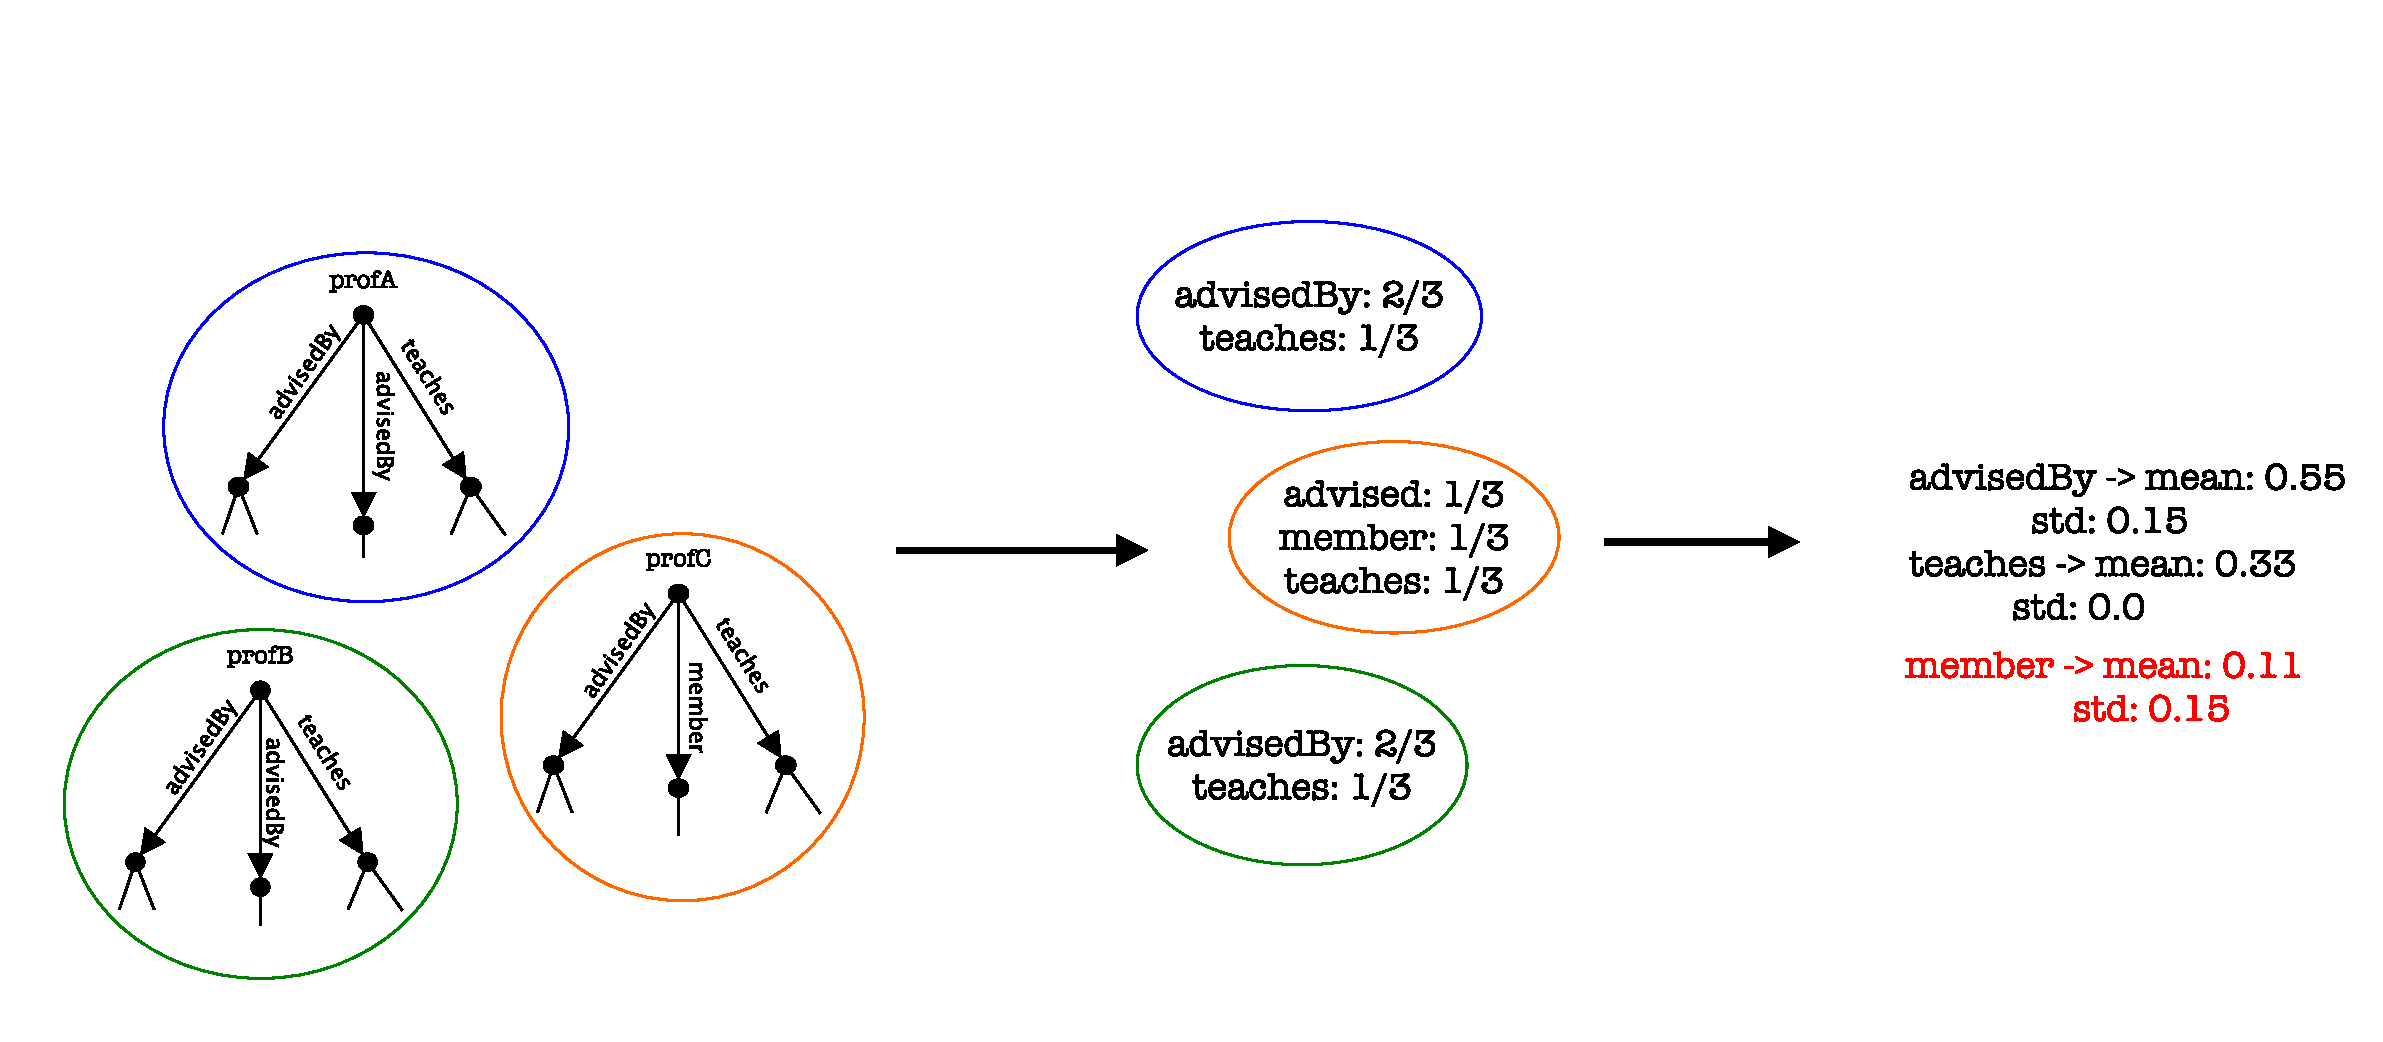
\includegraphics[width=.9\linewidth]{processIllustration}
    \caption[Discovering the meaning of latent features by analysing their relations]{\textbf{Discovering the meaning of latent features by analysing their relations.} Properties that describe latent features are the ones that have similar relative frequency in all neighbourhood trees. Starting from a cluster of instances viewed as neighbourhood trees (left), the relative frequencies of elements are calculated for each neighbourhood tree (middle). Next, the mean and standard deviation of relative frequencies are calculated for each individual element within the cluster (right). Which elements \textit{explain} the latent features is decided with $\theta$-confidence. Setting $\theta$ to 0.3 identifies \texttt{advisedBy} and \texttt{teaches} as relevant elements (in black).}
    \label{fig:Process}
\end{sidewaysfigure}





To identify such elements, we proceed in three steps illustrated in Figure~\ref{fig:Process}.
\begin{enumerate}
	\item \textbf{Calculate the relative frequencies of all elements within each individual neighbourhood tree, per level and vertex type}.
    	In case of discrete attributes, that corresponds to a distribution of its values.
		In case of numerical attributes, we consider its mean value.
		In case of vertex identities and edge types, we simply look into their frequencies with respect to the depth in a neighbourhood tree.
        In the example in Figure~\ref{fig:Process}, the neighbourhood tree for \texttt{profA} contains two \texttt{advisedBy} relations, thus its frequency is $\frac{2}{3}$.
    \item \textbf{Calculate the mean and standard deviation of relative frequency for each element within a cluster}.
        In Figure~\ref{fig:Process}, the frequencies of the \texttt{advisedBy} elements in individual neighbourhood trees are $\frac{2}{3}, \frac{2}{3} \text{and} \frac{1}{3}$. Thus, its mean is $0.55$ with a standard deviation of $0.15$.
    \item \textbf{Select relevant elements.}
    	The final step involves a decision which elements should form a definition of a latent feature.
        Relevant elements are identified by a notion of \textit{$\theta$-confidence} which captures the allowed amount of variance in order to element to be relevant.
\end{enumerate}


\begin{definition}{\textbf{($\theta$-confidence)}}
An element with mean value $\mu$ and standard deviation $\sigma$  in a cluster,  is said to be $\theta$-confident if $\sigma \in [0, \theta \cdot \mu]$.
\end{definition}

In Figure~\ref{fig:Process}, setting $\theta$ to 0.3 makes \texttt{advisedBy} a $0.3$-confident element, because its standard deviation of 0.15 is within the range $[0, 0.3 \cdot 0.55] = [0, 0.165]$ specified by $\theta$.
In contrast, \texttt{member} is not a $0.3$-confident elements as its standard deviation is outside the range $[0, 0.3 \cdot 0.11] = [0, 0.0363]$.


The above-described procedure explains the latent features in terms of distribution of the elements in the neighbourhood of an instance, which has its pros and cons.
On the downside, this type of explanation does not conform to the standard first-order logic syntax common within relational learning.
Despite this reduced readability, these explanations are substantially more transparent and interpretable than the ones produced by the embeddings approaches.
However, one benefit of this approach is that it increases the expressivity of a relational learner by extensionally defining  properties otherwise inexpressible in the first-order logic.


\subsection{A few examples}


%We devise the experiments to answer the following question:

 %\textit{Are latent features created by \gls{curled} interpretable and do they capture sensible information?}


%The results  obtained in \gls{curled} can be divided in three categories.
%The first category contains the IMDB and UWCSE datasets; these datasets present easy relational learning tasks in which the original data representation is sufficient for almost perfect performance.
%The main benefit of latent representations for these tasks was the reduction of model complexity.
%The second category includes the TerroristAttack dataset, in which the main benefit of latent representation was the reduction of complexity, but not the performance.
%The third category involves the Hepatitis, Mutagenesis and WebKB datasets.
%These tasks benefited from latent representations in both performance and reduced model complexity.
%That is especially true for the Hepatitis and WebKB datasets on which the performance was improved by a large margin.


%We take a representative task from each of the categories.
%Precisely, we use IMDB, UWCSE, Hepatitis and TerroristAttack datasets in our experiments.
%Both IMDB and UWCSE datasets were included as they are easy to understand without the domain knowledge, and thus useful for analysing the interpretability of relational latent features.
%As for the parameters of latent representation, we take the best parameters on individual datasets selected by the model selection procedure in \cite{Dumancic2017}.
%We set $\theta$ to $0.3$.


%\subsection{Interpretability}

\begin{figure}[t]
	\centering
	\medskip
    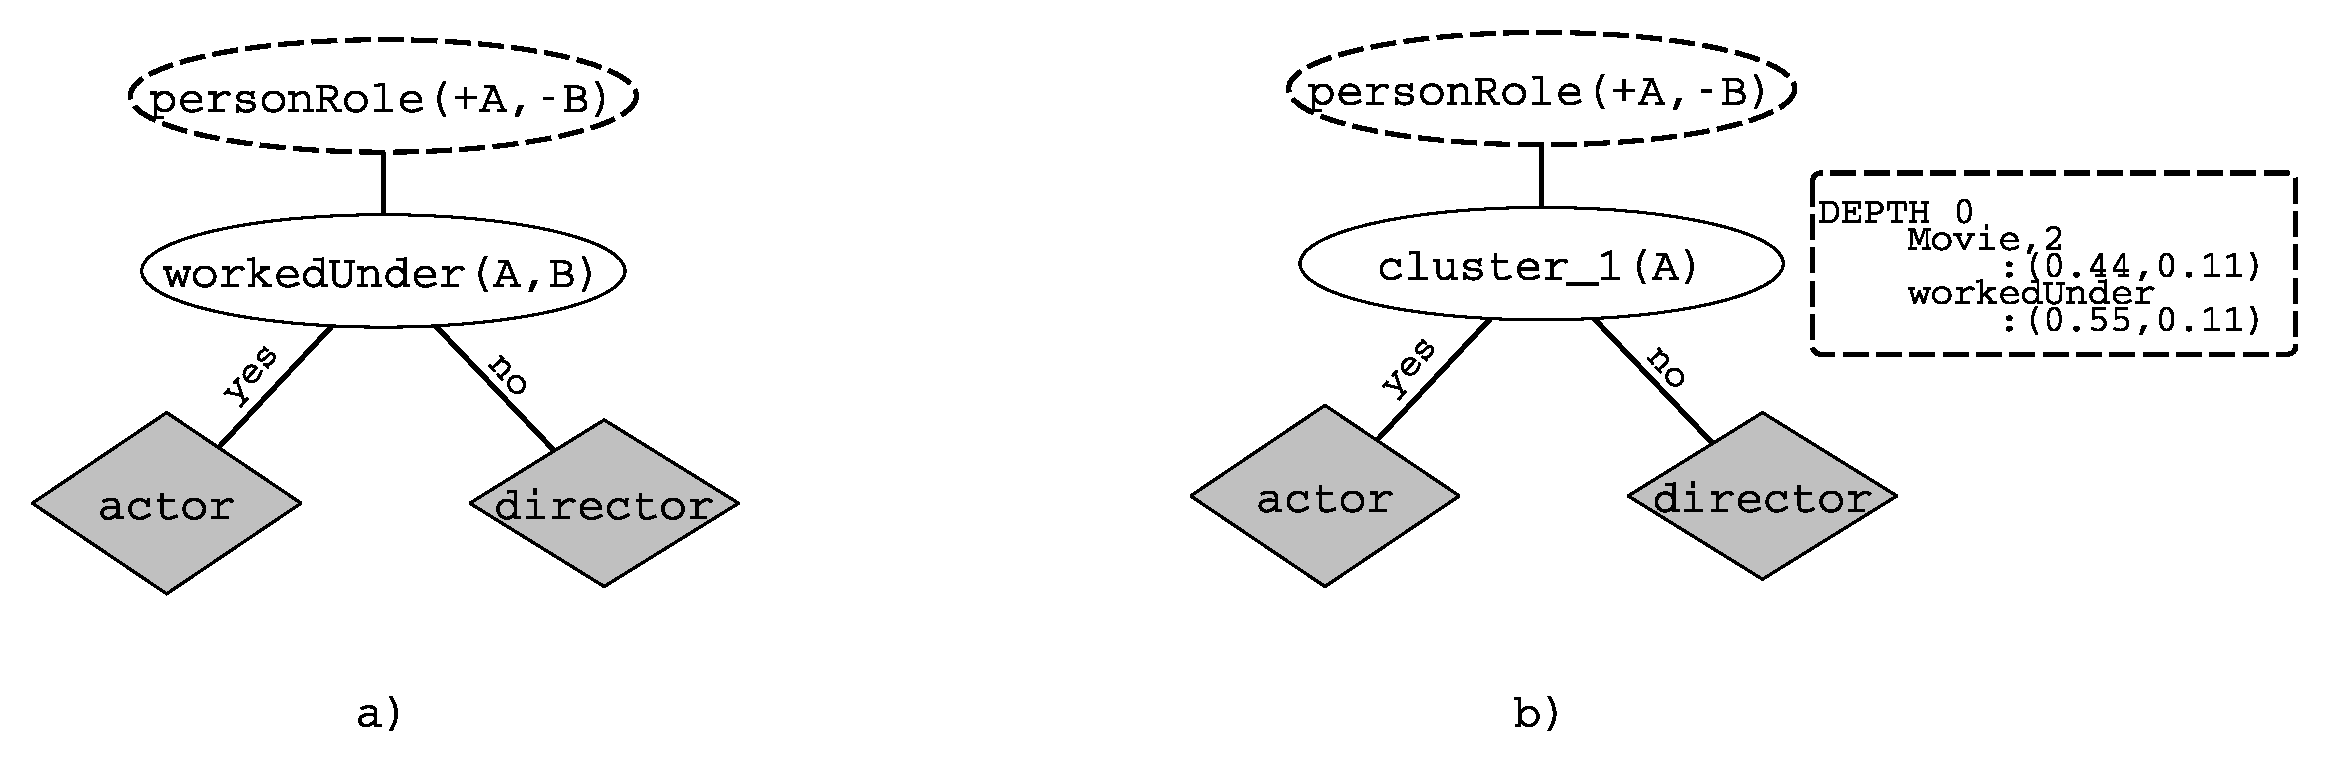
\includegraphics[scale=0.3]{IMDBtrees}
    \caption[Explanation of the latent features invented on the IMDB dataset]{Relational decision trees learned on the original (left) and latent (right) data representation of the IMDB dataset. The dashed ellipse indicates the target predicate and its arguments. The first argument, marked \texttt{A} and declared as input (\texttt{+}), denotes a person. The second argument, marked \texttt{B} and declared as output (\texttt{-}), states the label of the instance given by \texttt{A}. The values in the leaves of the decision trees are assignments to \texttt{B}. The dashed rectangle describes the latent feature -- for each level of the \textit{mean neighbourhood tree}, $\theta$-confident elements are listed with the mean and standard deviation.  }
    \label{fig:IMDBtree}
\end{figure}



To illustrate the interpretability of relational features, we show examples of latent features created for two easy to interpret dataset - IMDB and UWCSE.
We show that the relational decision trees  learned on both original and latent representations.
The explanations of latent features are provided as well.



Figure~\ref{fig:IMDBtree} shows the decision trees learned on the IMDB dataset.
The task is to distinguish between actors and directors -- this is a simple relational learning task and both original and latent decision tree achieve the perfect performance with only a single node.
Even though latent representation does not seem beneficial in this particular case, it is interesting to see that the selected latent feature captures the same information as the decision tree learned on the original data -- person instances in \texttt{cluster\_1} are the ones that have a relationship with \texttt{movie} instances, and have worked under another person (a director).



\begin{figure}[t]
	\centering
	\medskip
	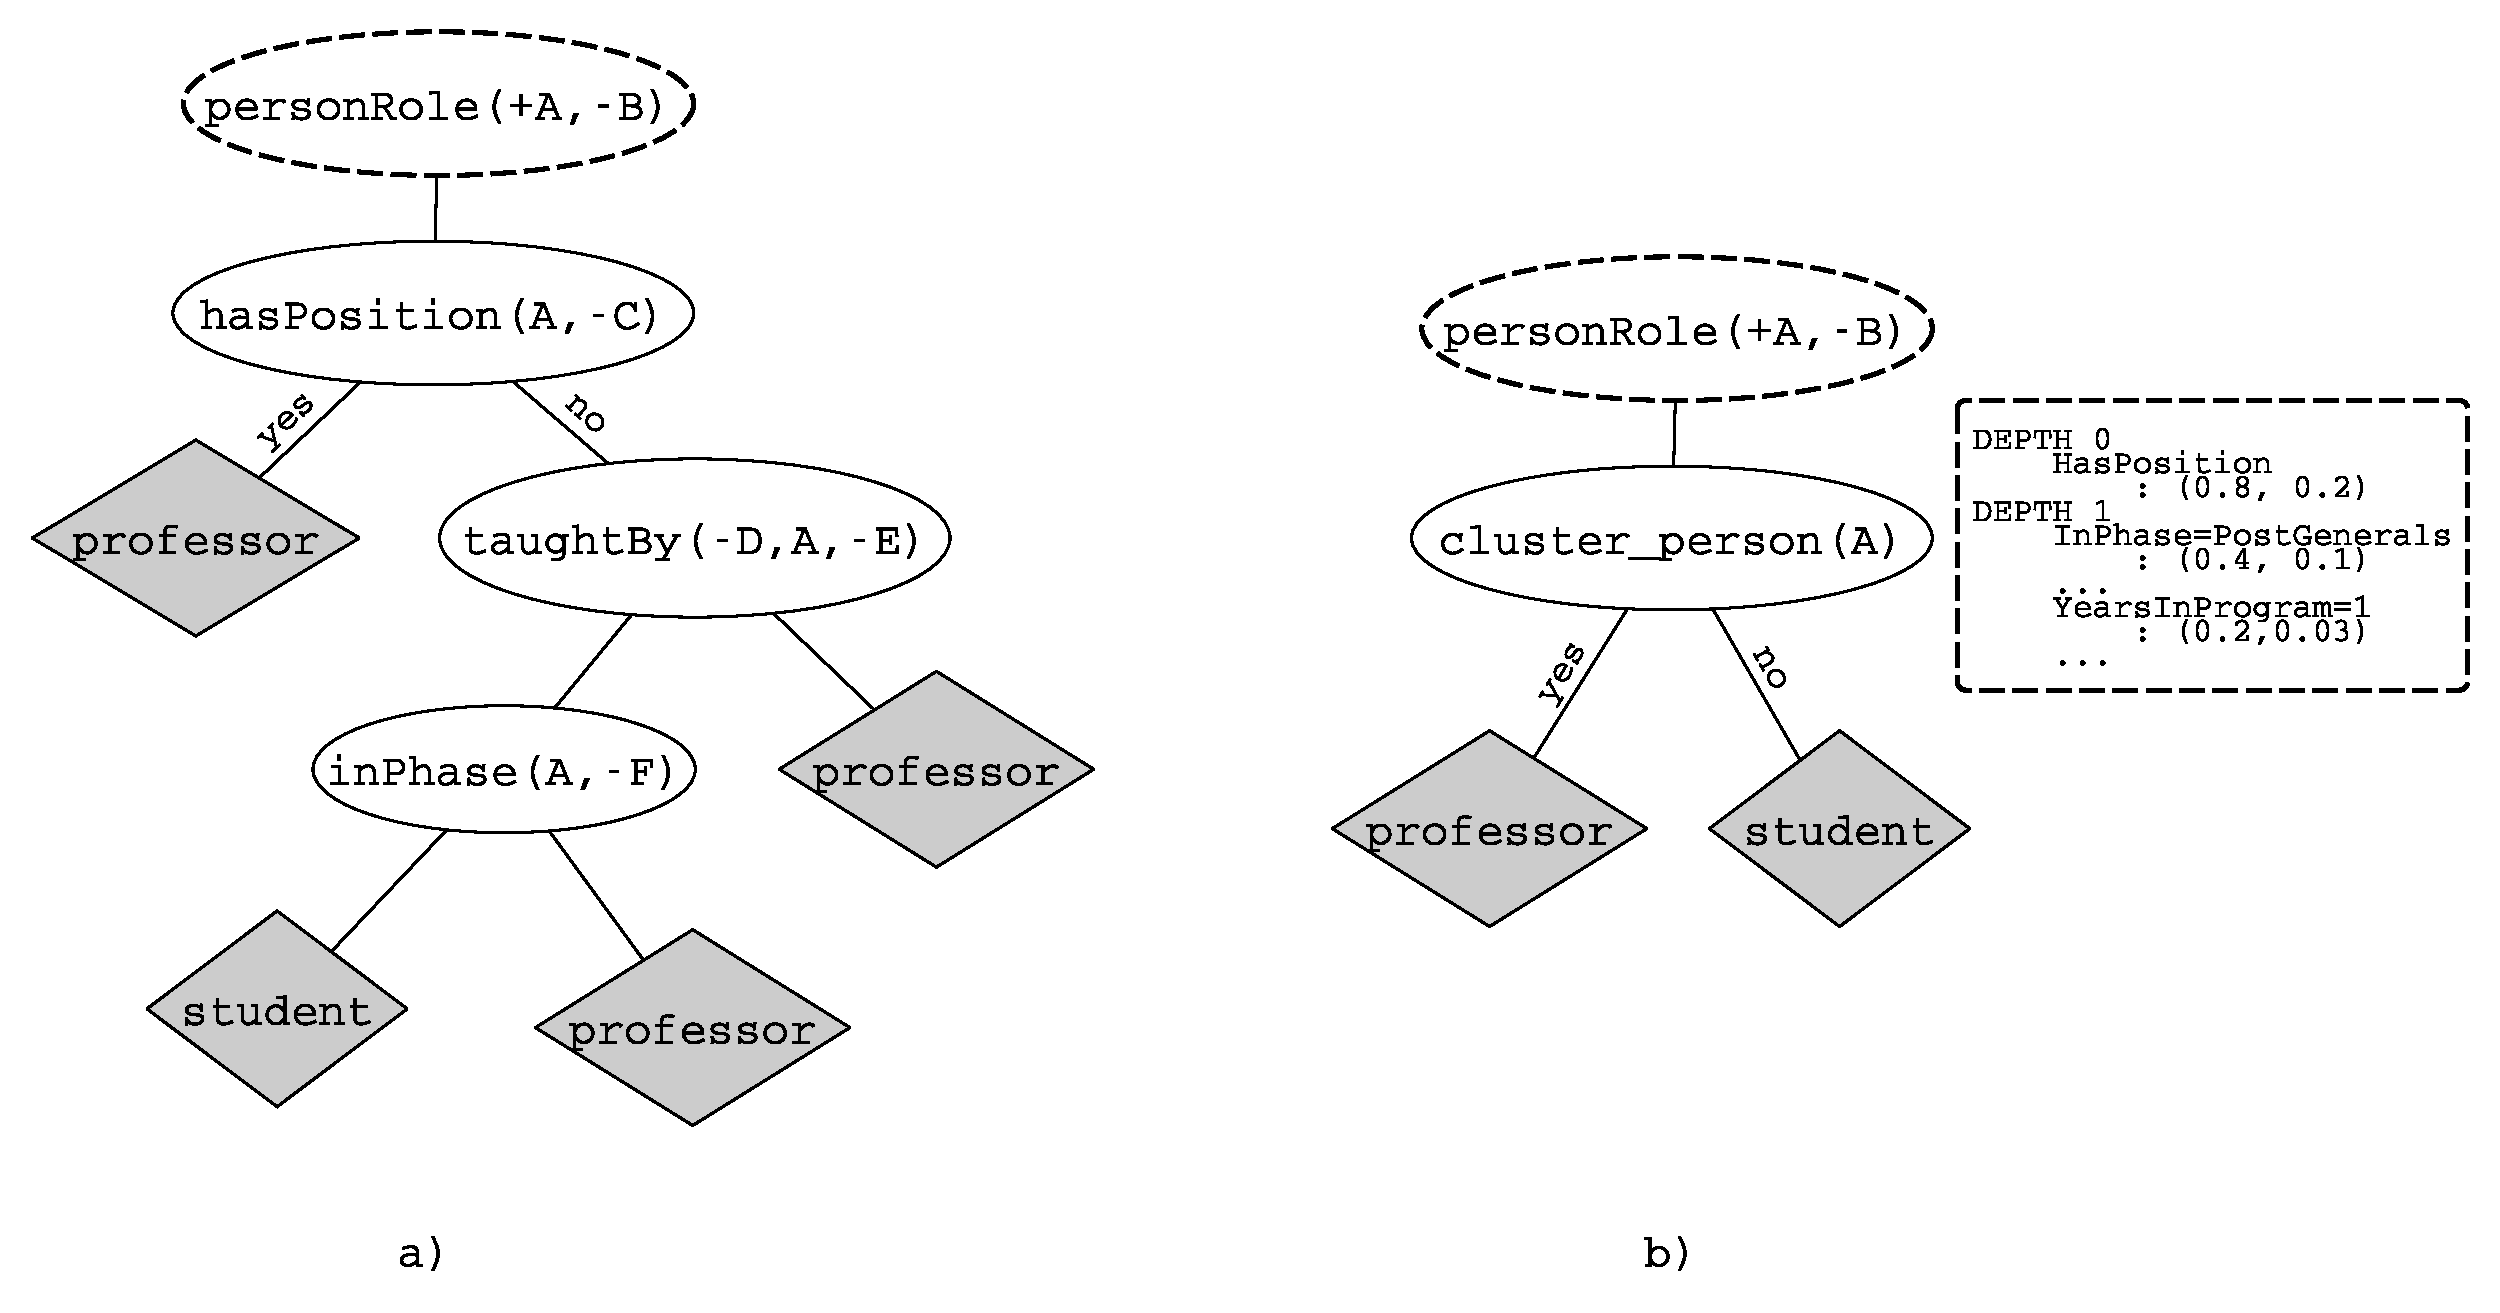
\includegraphics[scale=0.28]{UWCSEtrees}
    \caption[Explanation of the latent features invented for the UWCSE dataset]{Relational decision trees learned on the original (left) and latent (right) representations of the UWCSE dataset. The elements have the same meanings as in Figure~\ref{fig:IMDBtree}. }
    \label{fig:UWCSEtree}
\end{figure}



Figure~\ref{fig:UWCSEtree} shows the decision trees for the UWCSE dataset, which benefit from the latent features.
Despite the simplicity of distinguishing students from professors, the decision tree learned on the latent features is more compact and has only a single node whereas the decision tree learned on the original features consists of three nodes.
The latent feature here again captures similar knowledge as the original decision tree but expressed in a simpler manner -- professor is someone who either has a position at the faculty, or is connected to people who are currently in a certain phase of a study program and have been in the program for a certain number of years.




What is particularly interesting about the examples above is that, even though the latent features are created in an unsupervised manner, they match the provided label very well.
Moreover, they seem to almost perfectly capture the labelled information as only a few features are needed to outperform the decision tree learned on the original data representation.
This observation shows that \gls{curled} is indeed capturing sensible knowledge in the latent space.



Both aforementioned examples are easy to understand and interpret without an extensive domain knowledge.
The other tasks that have benefited more from the latent features are substantially more difficult to understand.
For instance, the latent features created from the Mutagenesis dataset reduce the complexity of the relational decision tree from 27 to only 3 nodes, while improving the accuracy for 4 \%.
Similarly, on the Hepatitis dataset the latent features reduced the complexity of a decision tree from 22 nodes down to 5, improving the accuracy for 11 \%.
Because these examples require an extensive knowledge to interpret them, we leave them out from this work.



\section{Conclusion}
\label{sec:Conc}


This chapter has introduces \gls{curled} - a clustering-based framework for unsupervised representation learning with relational data, which describes both instances and relationships between them.
Viewing relational data as hyper-graph, \gls{curled} learns new features by clustering both instances and their relationships. i.e., vertices and hyper-edges in the corresponding hyper-graph.
To support such procedure, we introduce a general hyper-edges clustering framework based on similarity of vertices participating in the hyper-edge.
A distinct feature of \gls{curled} is the way it uses different interpretations of similarity for relational data, i.e., whether two relational objects are similar due to their features of relationships, to generate a new data representation.
We design several experiments to verify the usefulness of latent representation generated by \gls{curled}.
The results show that the latent representations created by \gls{curled} provide a better representation of data that results in models of lower complexity and better performance.




%%%%%%%%%%%%%%%%%%%%%%%%%%%%%%%%%%%%%%%%%%%%%%%%%%
% Keep the following \cleardoublepage at the end of this file,
% otherwise \includeonly includes empty pages.
\cleardoublepage

% vim: tw=70 nocindent expandtab foldmethod=marker foldmarker={{{}{,}{}}}
